\chapter{\en{Virtual Environment Set up}}

\section{\en{GNS3 Installation}}

Το \en{GNS3} είναι ένα λογισμικό που χρησιμοποιείται για την εξομοίωση, τη διαμόρφωση και τη δοκιμή ενός περιβάλλοντος δικτύου. Είναι
είναι ένα ελεύθερο λογισμικό ανοικτού κώδικα και μπορείτε να το κατεβάσετε από τον επίσημο δικτυακό τόπο 
\en{https://www.gns3.com/} .Το \en{GNS3} αποτελείται από δύο στοιχεία. Το ολοκληρωμένο λογισμικό (\en{GUI}) το οποίο είναι ένα γραφικό 
διεπαφή χρήστη και την εικονική μηχανή (\en{VM}), η οποία είναι ένας διακομιστής που εκτελείται σε εικονικό περιβάλλον και παρέχει καλύτερο μέγεθος τοπολογίας και υποστήριξη συσκευών.
Η εγκατάσταση είναι απλή και θα πρέπει να χρησιμοποιούνται οι προεπιλεγμένες επιλογές.

Για να γίνει σωστά η εγκατάσταση θα πρέπει το \en{software version} του \en{GNS3} να είναι το ίδιο με το
\en{software version} του \en{GNS3 VM}. Όταν λοιπόν γίνει η εγκατάσταση και ανοίγουμε το \en{GNS3 GUI}
αυτή η ενέργεια θα κάνει \en{trigger} το \en{booting} του \en{GNS3 VM}
Μόλις γίνει η εγκατάσταση μπορεί να ανοίξει η εφαρμογή και να κάνουμε \en{import cisco IOS images}. Στην παρακάτω
εικόνα μπορούμε να δούμε τι γίνεται όταν ανοίγουμε το \en{GNS3}. 

\begin{figure}[h]
	\centering
	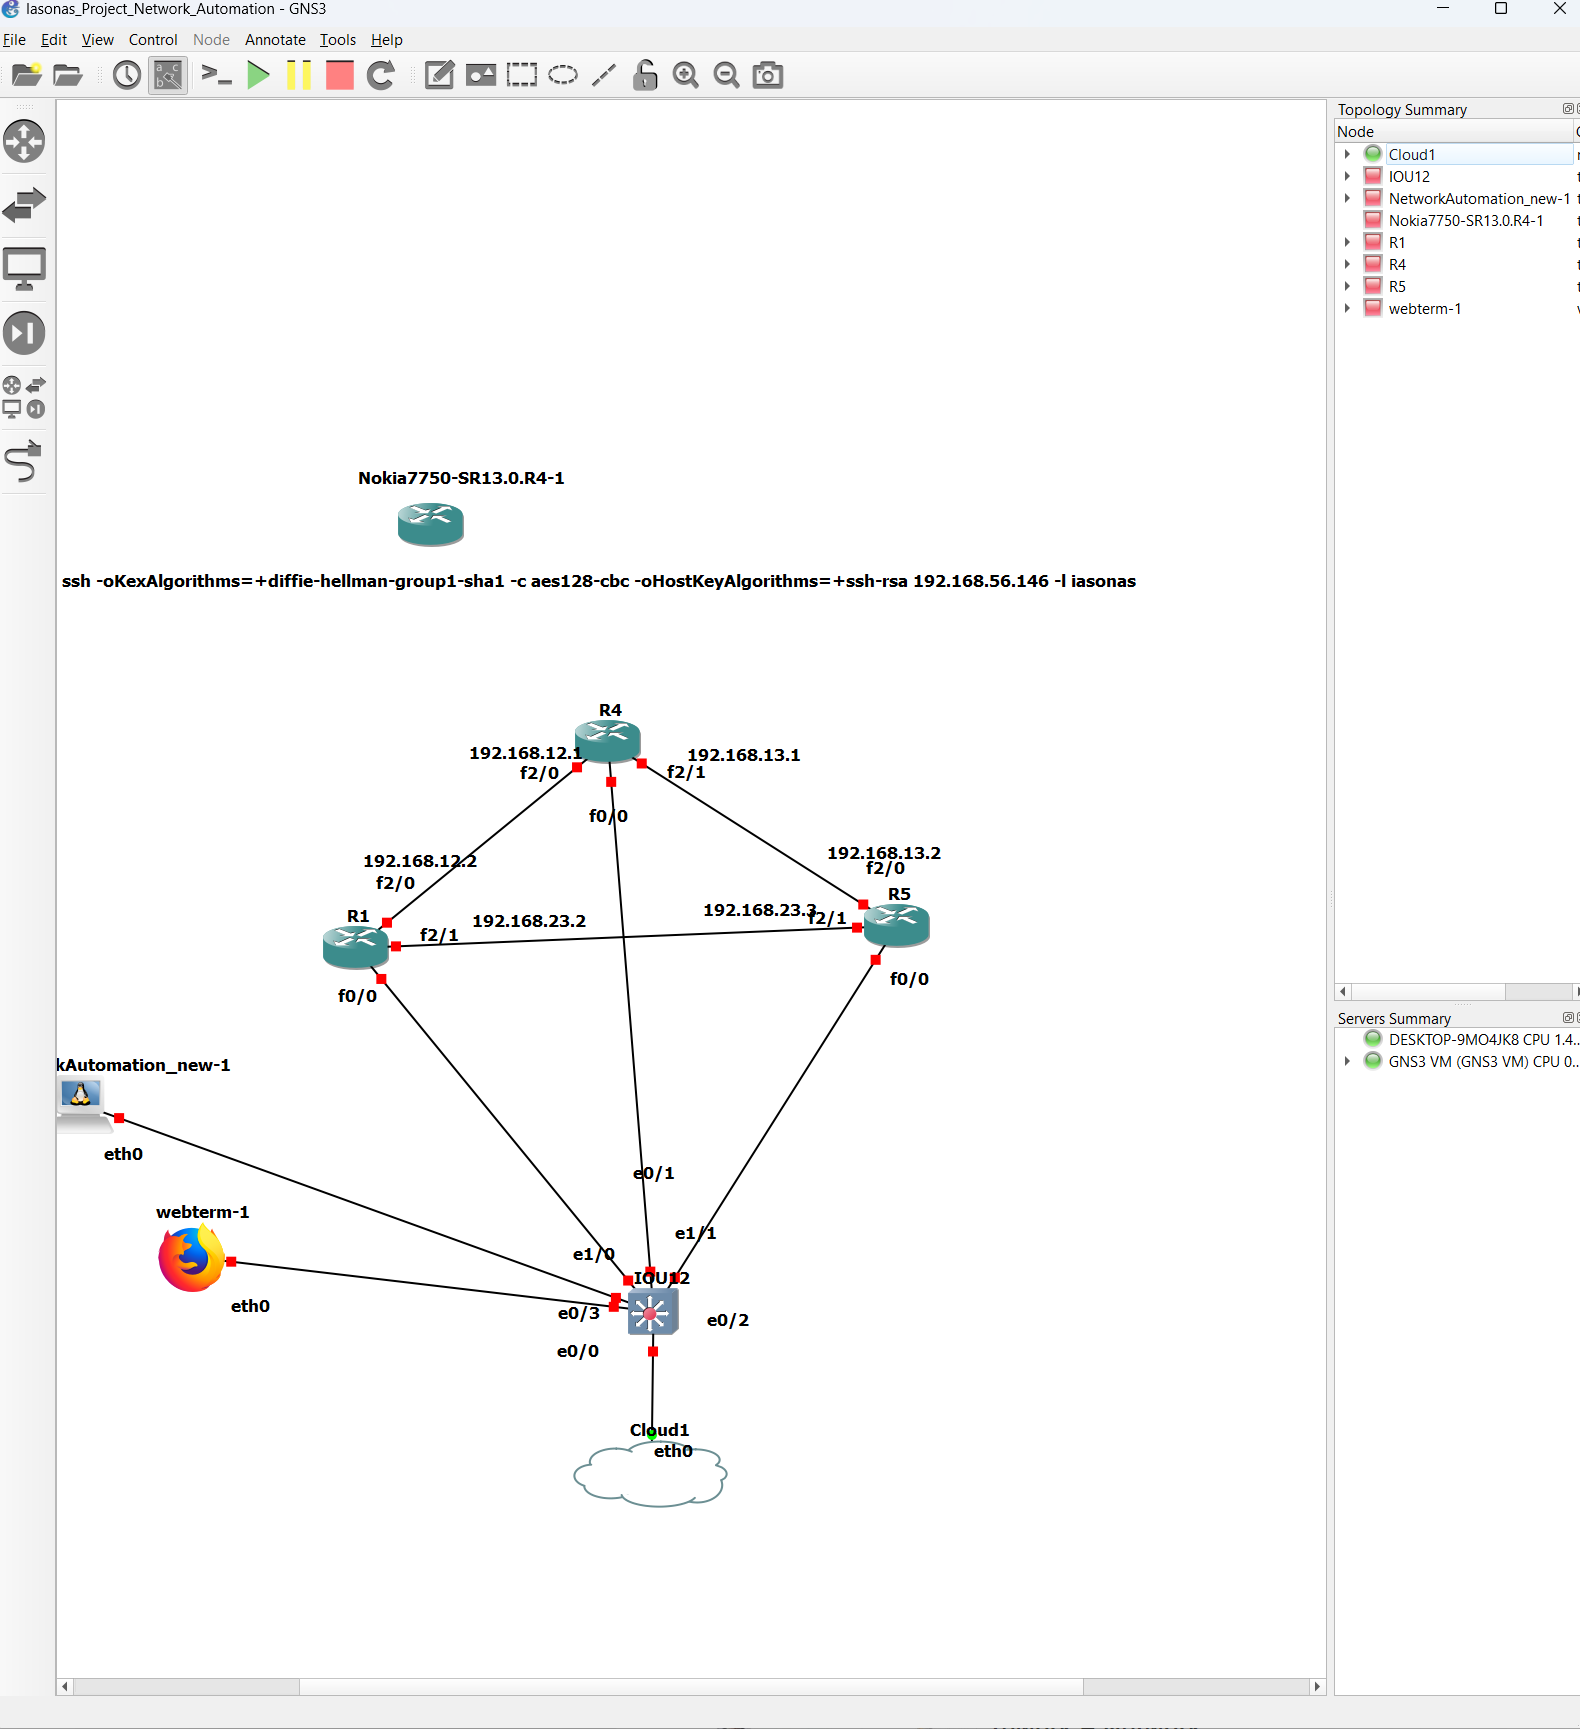
\includegraphics[width=0.7\textwidth]{graphics/gns3_homepage.png}
	\caption{\en{GNS3 homepage} }
\end{figure}

\FloatBarrier

Προκειμένου να μπορέσει να επικοινωνήσει το \en{PC} μας στο τοπικό δίκτυο με το \en{GNS3 VM} στο τοπικό δίκτυο
θα πρέπει να γίνουν κάποιες ρυθμίσεις τόσο στο \en{GNS3 VM} όσο και στις συσκευές της \en{Cisco}

Στις συσκευές της \en{Cisco} θα πρέπει να γίνει η παρακάτω παραμετροποίηση όπως εμφανίζεται στις εικόνες 4.1,4.2,4.3.

\begin{figure}[h]
	\centering
	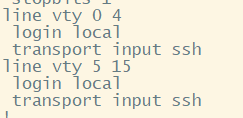
\includegraphics[width=0.7\textwidth]{graphics/cisco_ssh_config.png}
	\caption{\en{Cisco ssh config} }
\end{figure}

\FloatBarrier

\begin{figure}[h]
	\centering
	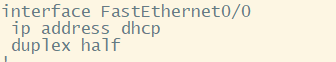
\includegraphics[width=0.7\textwidth]{graphics/dhcp_cisco_config.png}
	\caption{\en{Cisco dhcp config} }
\end{figure}

\FloatBarrier

Μέχρι αυτή τη στιγμή έχουμε παραμετροποιήσει τις συσκευές με τέτοιο τρόπο ώστε να δέχονται
απομακρυσμένη σύνδεση. Τώρα θα εξηγήσουμε πως μπορούμε να φτιάξουμε την εποικοινωνία μεταξύ εικονικών
μηχανών της \en{Cisco} και του τοπικού μας υπολογιστή. Η λογική είναι ότι η συσκευή \en{Cloud}
θα μας επιτρέψει να φτιάξουμε τη σύνδεση αυτή. Η εικόνα 4.4 μας παρουσιάζει σε ανώτερο επίπεδο τη λογική αυτή σύνδεση.

\FloatBarrier

\begin{figure}[htb]
	\centering
	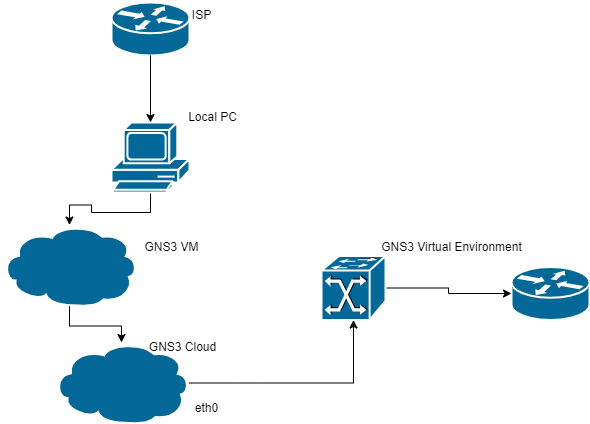
\includegraphics[width=0.7\textwidth]{graphics/diagram.drawio.png}
	\caption{\en{Local PC-GNS3VM-CISCO IOS Connection Architecture} }
\end{figure}









\section{\en{Connection Establishment} }


Μετά την ολοκλήρωση της παραμετροποίησης και της διαμόρφωσης της τοπολογίας, όλα τα διαφορετικά στοιχεία (\en{components}) 
θα πρέπει να ανήκουν στο ίδιο τοπικό δίκτυο. Η εικονική διεπαφή μέσω της οποίας θα διέρχεται όλη η δικτυακή κίνηση, είτε πρόκειται για \en{REST}
είτε για \en{SSH}, είναι η διεπαφή \en{eth0} στο περιβάλλον του \en{GNS3 VM}. Στην εικόνα 4.6 παρατίθεται ένα αρχείο καταγραφής (\en{trace}), 
το οποίο επιβεβαιώνει ότι η σύνδεση πραγματοποιείται απρόσκοπτα.

Η βασική απαίτηση είναι η διεπαφή μεταξύ του \en{GNS3 VM} και του τοπικού υπολογιστή να ανήκουν στο ίδιο δίκτυο. 
Για να επιτευχθεί αυτό, εφαρμόστηκε η κατάλληλη παραμετροποίηση στο \en{GNS3 VM}, όπως παρουσιάζεται στο Σχήμα 4.5. 
Με αυτόν τον τρόπο, εφόσον το \en{GNS3 VM} έχει ενταχθεί στο τοπικό δίκτυο, το ίδιο μπορεί να συμβεί και για τις συσκευές της \en{Cisco}
, οι οποίες θα εισαχθούν στο περιβάλλον εργασίας μας, επιτρέποντας τη διαδραστικότητα και την επικοινωνία με αυτές.


\begin{figure}[htb]
	\centering
	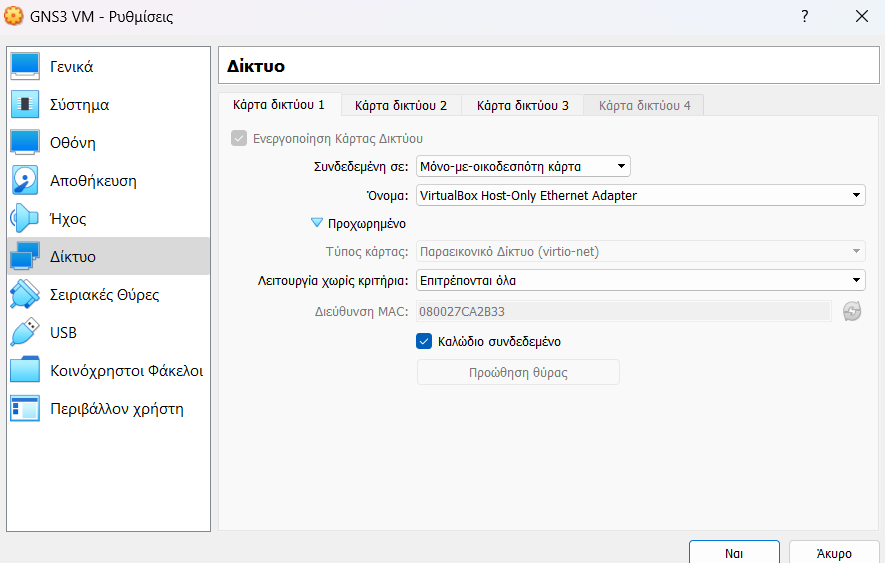
\includegraphics[width=1.0\textwidth]{graphics/network_config_GNS3.png}
	\caption{\en{Network Configuration for GNS3VM} }
\end{figure}

\FloatBarrier

\begin{figure}[htb]
	\centering
	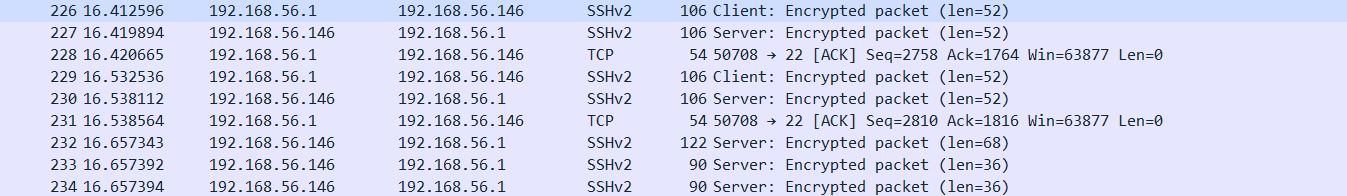
\includegraphics[width=1.0\textwidth]{graphics/ssh_connection.png}
	\caption{\en{SSH traffic} }
\end{figure}


Προκειμένου να γίνει η συλλογή του συγκεκριμένου \en{trace} χρησιμοποιήθηκε η παρακάτω εντολή:
\en{ tcpdump -i eth0 -v -w /home/gns3/test.pcap}
.Η συλλογή του \en{trace} έγινε με το πρωτόκολλο \en{SFTP}.

\FloatBarrier

\begin{figure}[h]
	\centering
	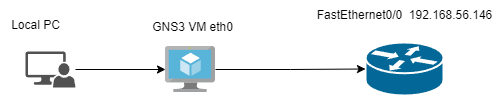
\includegraphics[width=0.7\textwidth]{graphics/jason1.png}
	\caption{\en{SSH traffic} }
\end{figure}

\FloatBarrier

\section{Σύνδεση με \en{Django Server} }

Ο \en{Django Server} τρέχει στον τοπικό υπολογιστή. Μπορεί να τρέξει σε οποιοδήποτε
μηχάνημα είναι \en{Linux} είτε \en{Windows} αρκεί να είναι στο τοπικό δίκτυο
είτε να υπάρχει κάποια συσκευή \en{layer2} η οποία να αναλάβει τη σύνδεση στο λεγόμενο
\en{data link layer}.


\section{Δομή της διαδικτυακής εφαρμογής \en{Django} }


\subsection{Τα αρχεία \en{urls.py}}
Τα αρχεία αυτά καθορίζουν τη δρομολόγηση των \en{URL} της εφαρμογής. 
Οι διευθύνσεις \en{URL} που αντιστοιχούν στα μοτίβα που περιγράφονται στο αρχείο \en{urls.py} 
προωθούνται στην αντίστοιχη συνάρτηση στο αρχείο \en{views.py}. 
Η αντιστοίχιση πραγματοποιείται σειριακά από πάνω προς τα κάτω στο αρχείο \en{urls.py}. 
Παρόλο που σε αυτό το έργο υλοποιήθηκε ακριβής αντιστοίχιση των \en{URL}, το \en{Django} παρέχει τη 
δυνατότητα χρήσης ταυτοποίησης μέσω κανονικών εκφράσεων. Στην εικόνα που ακολουθεί, παρουσιάζονται οι 
διευθύνσεις \en{URL} του \en{API}, όπου κάθε διεύθυνση αντιστοιχεί σε μια συνάρτηση στο αρχείο \en{api1/views.py}, 
η οποία καταλήγει στην εκτέλεση του αντίστοιχου σεναρίου

\begin{figure}[htb]
	\centering
	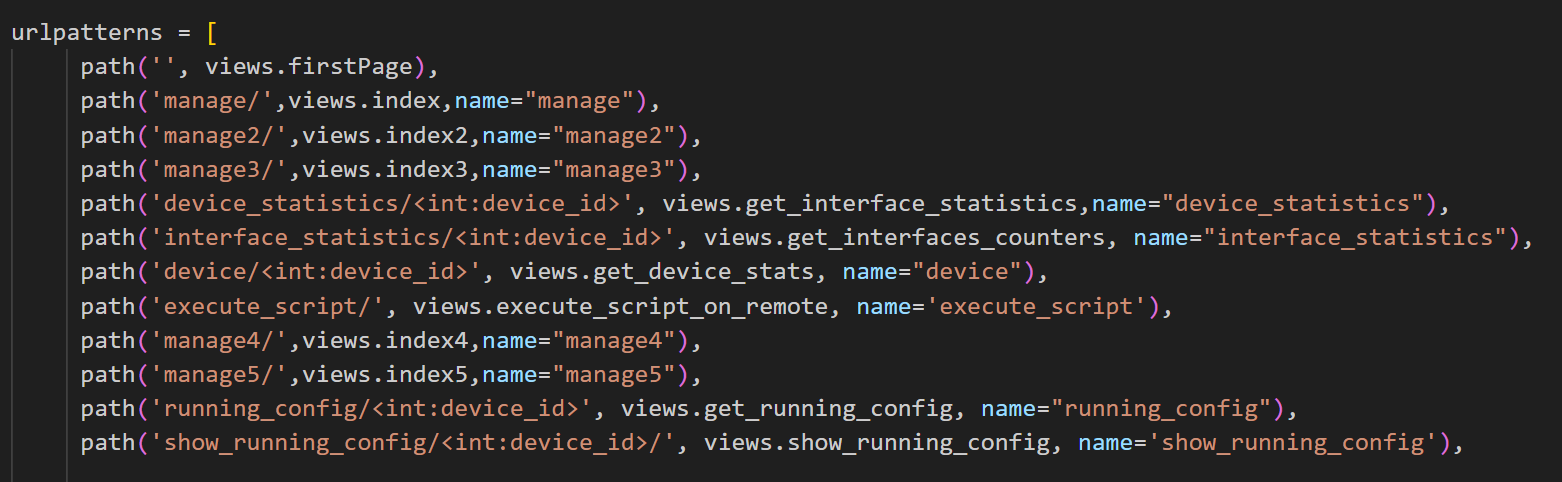
\includegraphics[width=0.9\textwidth]{graphics/urlpy.png}
	\caption{\en{url.py} }
\end{figure}

\subsection{Τα αρχεία \en{views.py}}

Οι συναρτήσεις σε ένα αρχείο \en{views.py} καλούνται όταν η δεδομένη διεύθυνση \en{URL} που αποστέλλεται από το
χρήστη ταιριάζει με το αντίστοιχο μοτίβο \en{URL} στο αρχείο \en{urls.py}. Παράμετροι που αποστέλλονται μέσω κλήσης
\en{HTTP} εισέρχονται στην αντίστοιχη συνάρτηση μέσω παραμέτρων ή σώματος αίτησης. Στο αρχείο \en{views.py} του \en{API}, η συνάρτηση εκτελεί το σενάριο
κώδικα με τις δεδομένες παραμέτρους εισόδου. Όταν τελειώσει η εκτέλεση του κώδικα δέσμης ενεργειών,
το αποτέλεσμα επιστρέφεται στη συνάρτηση \en{views} και μεταβιβάζεται ως πλαίσιο στο αντίστοιχο αρχείο \en{.html} για την εμφάνιση των αποτελεσμάτων στον χρήστη που εκτέλεσε το σενάριο.
Ένα παράδειγμα μιας συνάρτησης σε ένα αρχείο en{views.py} μπορείτε να δείτε στο σχήμα παρακάτω

\begin{figure}[htb]
	\centering
	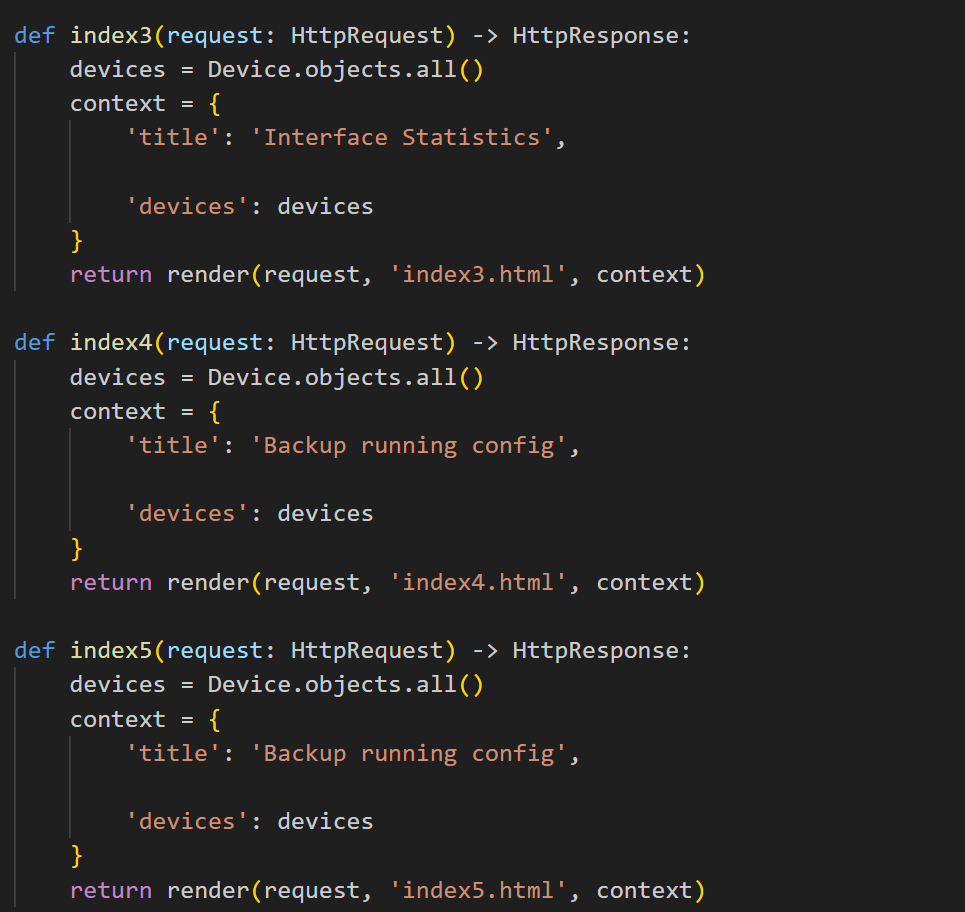
\includegraphics[width=0.9\textwidth]{graphics/viewspy.png}
	\caption{\en{views.py} }
\end{figure}

\subsection{Τα αρχεία \en{html template}}

Στη συνάρτηση \en{views.py}, το \en{Django} αποδίδει το αντίστοιχο πρότυπο \en{.html}
αρχείο με ένα συγκεκριμένο πλαίσιο. Το πλαίσιο είναι σε μορφή \en{JavaScript Object Notation (JSON)} και αποστέλλεται στο αρχείο \en{.html}. Τα δεδομένα στο πλαίσιο εμφανίζονται
στο \en{.html}, εάν το \en{.html} έχει παραμετροποιηθεί κατάλληλα. Ένα παράδειγμα \en{.html} με
τον συντακτικό κώδικα για τον τρόπο πρόσβασης στα δεδομένα του πλαισίου παρουσιάζεται στην εικόνα παρακάτω



\begin{figure}[htb]
	\centering
	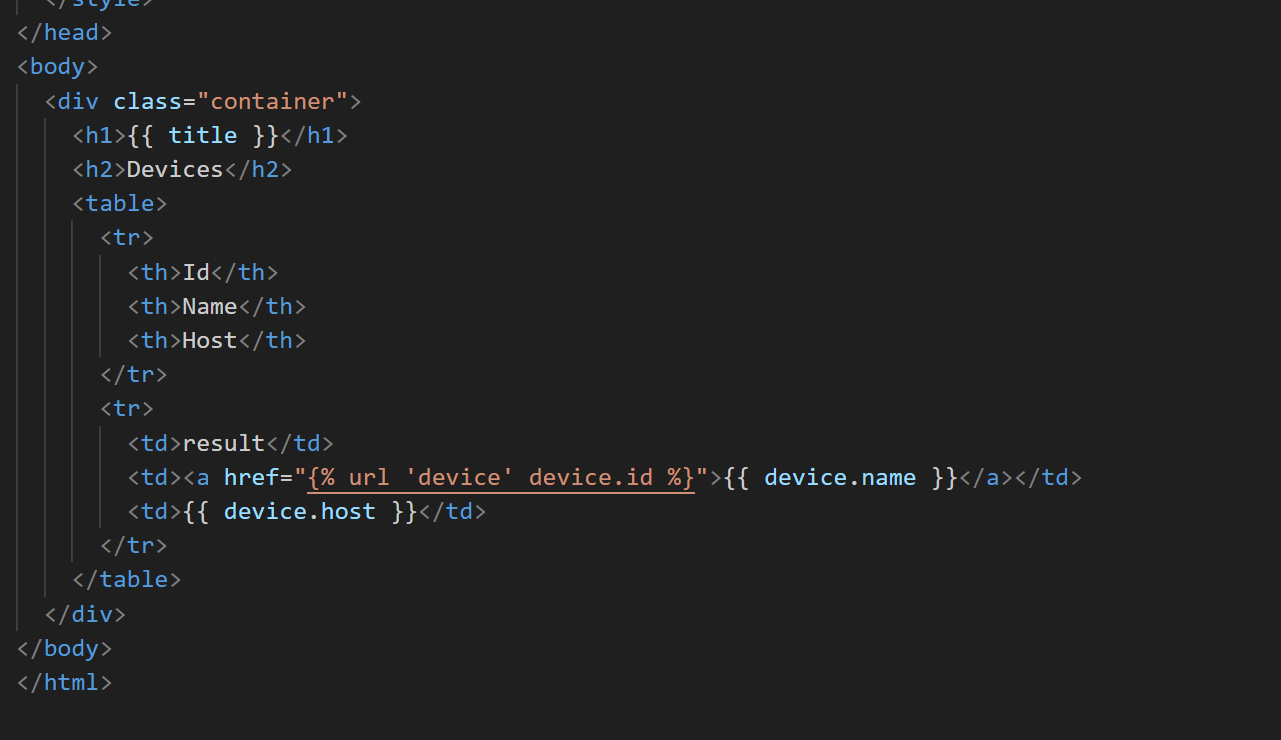
\includegraphics[width=0.9\textwidth]{graphics/html_template.png}
	\caption{Παράδειγμα \en{html} αρχείου }
\end{figure}






\subsection{Η βάση δεδομένων}
Η διαδικτυακή πύλη χρησιμοποιεί μια βάση δεδομένων \en{SQLite}. Αυτή η βάση δεδομένων περιέχει τρία
μοντέλα τα οποία ορίζονται στο αρχείο \en{models.py}. Το αρχείο αυτό περιέχει μία κλαση Device η οποία δέχεται σαν ορίσματα
το όνομα, την \en{IP}, το όνομα χρήστη, τον κωδικό, τον κρυφό κωδικό και το μοντέλο της συσκευής.
Υπάρχει μία εγγραφή στη βάση δεδομένων ένα από αυτά τα αντικέιμενα τα οποία εμείς τα δημιουργούμε. Το μοντέλο διαπιστευτηρίων αποθηκεύει τα διαπιστευτήρια τα οποία έχουν προηγουμένως
κρυπτογραφημένα. Με αυτό, ορισμένες δέσμες ενεργειών μπορούν να λάβουν τα διαπιστευτήρια που απαιτούνται για να λειτουργήσουν
χωρίς την είσοδο του χρήστη και χωρίς να γίνεται άμεση αναφορά στα διαπιστευτήρια στο
κώδικα.
Η διαχείριση της βάσης δεδομένων μπορεί να γίνει απευθείας μέσω μιας γραφικής διεπαφής χρήστη
\en{(GUI)} στο \en{Django}. Σε αυτό το \en{GUI} μπορούν να έχουν πρόσβαση μόνο οι χρήστες διαχειριστές. Παραδείγματα
των εγγραφών του μοντέλου της εφαρμογής  που εμφανίζονται σε αυτό το \en{GUI} παρουσιάζονται παρακάτω στην εικόνα.

\begin{figure}[htb]
	\centering
	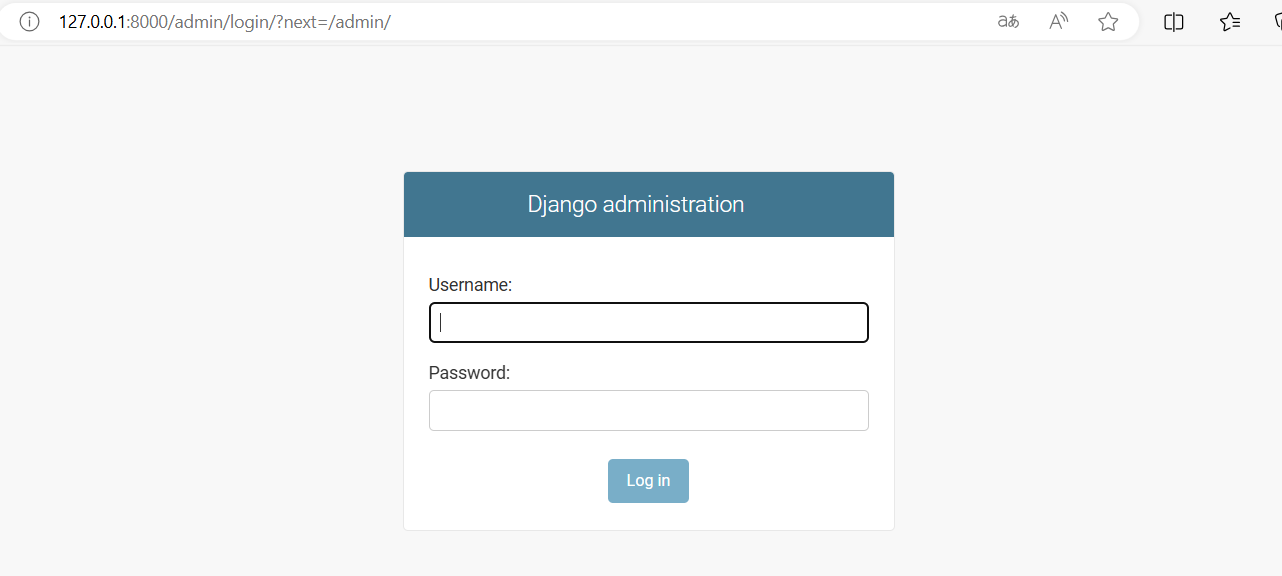
\includegraphics[width=0.9\textwidth]{graphics/GUI_LOGIN.png}
	\caption{Είσοδος στο \en{GUI}}
\end{figure}

\begin{figure}[htb]
	\centering
	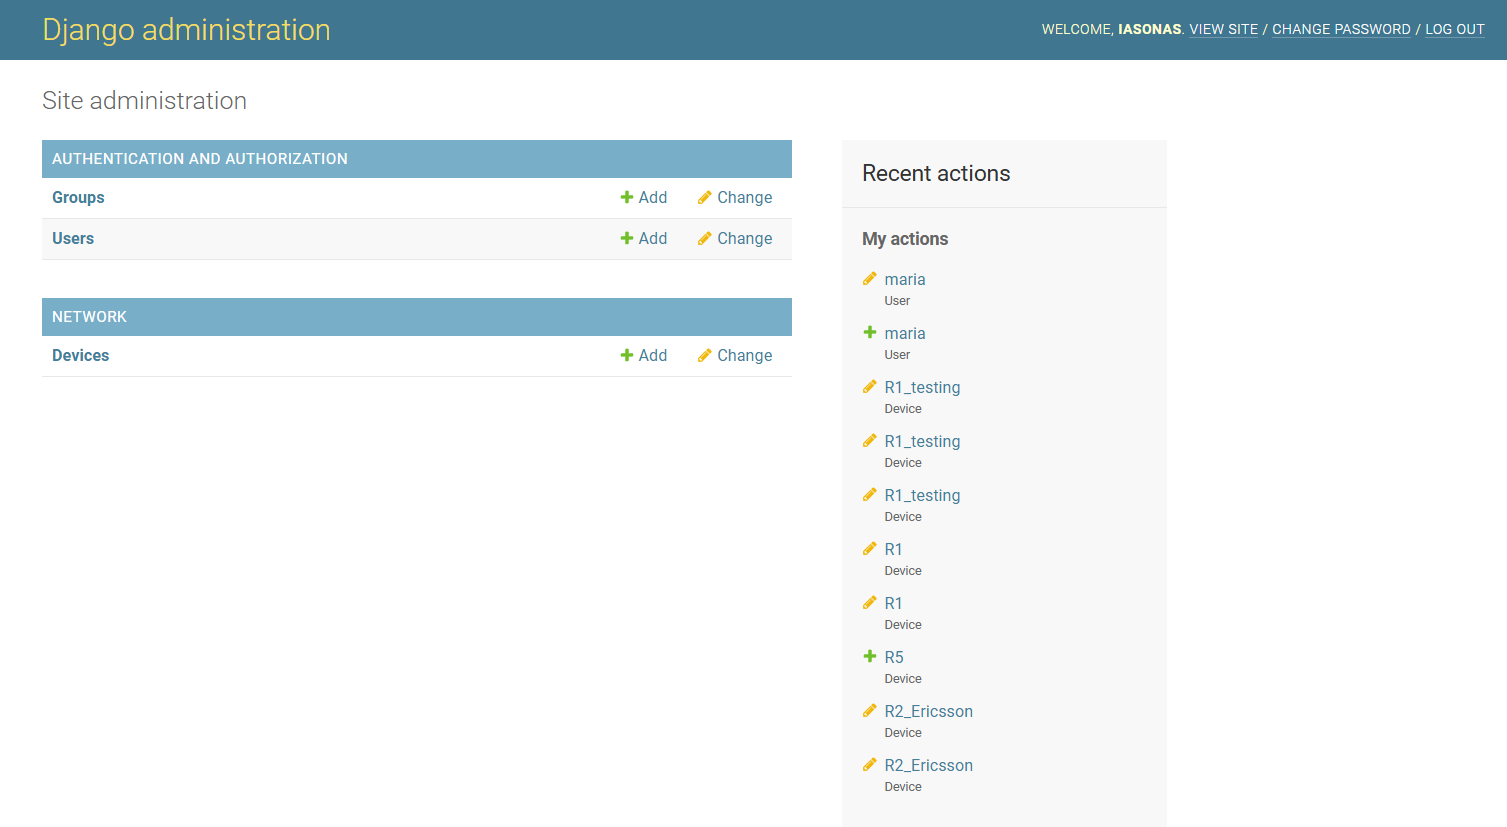
\includegraphics[width=0.9\textwidth]{graphics/DJANGO_ADMIN.png}
	\caption{Κεντρική σελίδα του \en{Django Administration GUI}}
\end{figure}

\begin{figure}[htb]
	\centering
	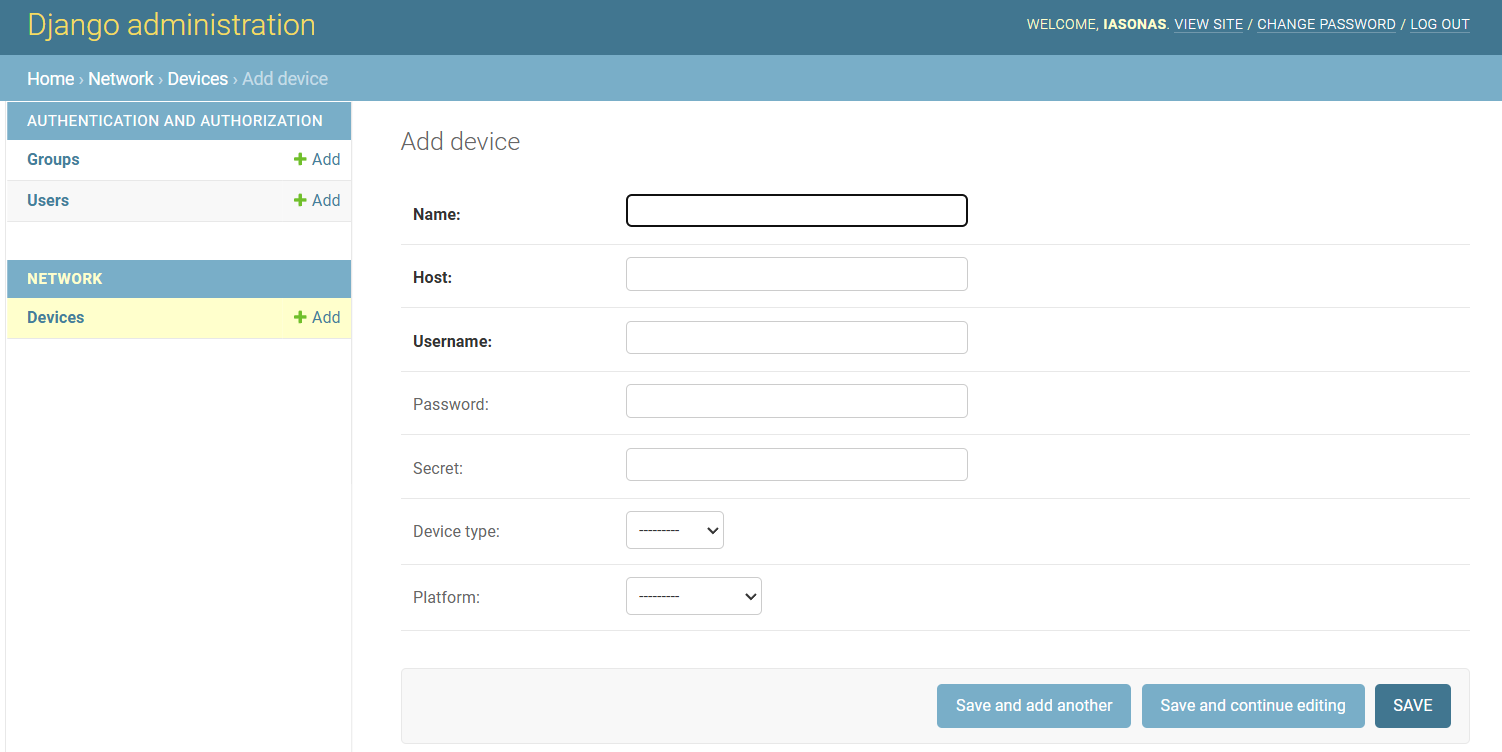
\includegraphics[width=0.9\textwidth]{graphics/ADD_DEVICE.png}
	\caption{Προσθήκη συσκευής }
\end{figure}


 Η προσθήκη συσκευής γίνεται συμπληρώνοντας στοιχεία όπως η \en{IP} διεύθυνση, το \en{username}, το \en{password} ,\en{secret} και το όνομα. Αν δώσουμε αυτά τα στοιχεία
 μετά το λογισμικό θα μπορέσει να κάνει τη δουλειά προκειμένου να μπει στη συσκευή και να εκτελέσει βασικές λειτουργίες που θα παρουσιάσουμε και παρακάτω. 







 
